\documentclass{article}
\usepackage[margin=1.2in]{geometry}
\usepackage{datetime}
%\usepackage{hyperref}      %for \url macro
\usepackage{microtype}     %attempt to fix issue with justification protrusion (in references)
\usepackage{amssymb}       % for formatting less/greater than symbols
\usepackage{amsmath}
\usepackage{enumitem}      %for changing spacing in bulleted lists
\usepackage{subfigure}        %for subfigures


\renewcommand{\arraystretch}{1.25}

\usepackage[gobble=auto, runall=true]{pythontex}
\usepackage{float} %for forcing position of images

\usepackage{graphicx}
\graphicspath{ {../images/} }
\usepackage[export]{adjustbox}
\usepackage[justification=centering]{caption}

\usepackage{listings}   %for typesetting code
\usepackage{color}
\definecolor{codegreen}{rgb}{0,0.6,0}
\definecolor{codegray}{rgb}{0.5,0.5,0.5}
\definecolor{codepurple}{rgb}{0.58,0,0.82}
\definecolor{backcolour}{rgb}{0.95,0.95,0.92}
\lstdefinestyle{mystyle}{
    backgroundcolor=\color{backcolour},
    commentstyle=\color{codegreen},
    keywordstyle=\color{codepurple},
    numberstyle=\tiny\color{codegray},
    stringstyle=\color{codepurple},
    basicstyle=\footnotesize,
    breakatwhitespace=false,
    breaklines=true,
    captionpos=b,
    keepspaces=true,
    %numbers=left,
    numbersep=5pt,
    showspaces=false,
    showstringspaces=false,
    showtabs=false,
    tabsize=2
}
\lstset{style=mystyle}

\frenchspacing                   %removes extra spacing after a period at the end of a sentence.
\newdateformat{daymonthyear}{
  \THEDAY\ \monthname\ \THEYEAR}

\title{CSC411 Machine Learning \\ Project 2: Deep Neural Network}
\author{ Ariel Kelman \\ Student No: 1000561368
         \\ \\
         Gideon Blinick \\ Student No: }
\daymonthyear



\begin{document}
   \maketitle{}


   \section{Introduction}
   The following figure shows 10 random images from the training set of each of the digits.
   \begin{figure}[H] \centering
      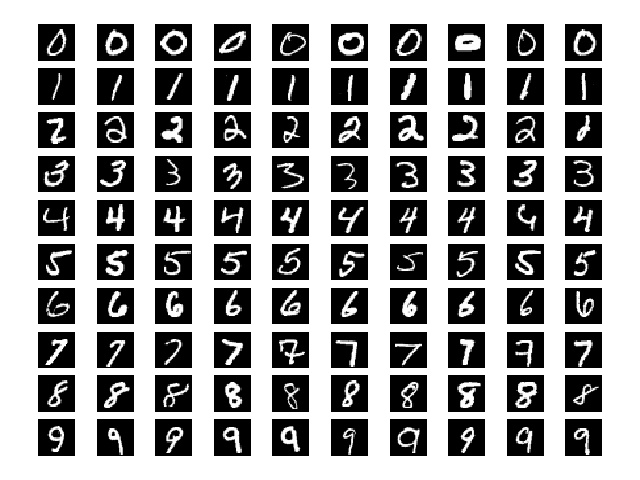
\includegraphics[width=4in]{resources/part1}
      \caption{10 random samples from the training set for each digit. This image
         was generated using \texttt{plot\_samples()}. }
   \end{figure}
   The data was downloaded from the assignment webpage, and imported into Python using the
   provided code. The data was already divided into training and testing sets...

   All results and plots can be generated using the python file...
   To reproduce the report, simply run it through latex.


   \section{The Network}
   The following function implements a neural network with no hidden layers, with the
   output passed through a softmax layer to estimated probabilities.

   \begin{lstlisting}[language=Python]
      def func():
   \end{lstlisting}

   The network is described by the weights and biases from the 784 = 28*28 inputs
   (representing pixel intenisites of the input image) to ten ``output'' nodes
   (with the identity as the activation function). The output from this layer is what is
   passed through the sofmax function $p_k = \frac{ e^{o_k} }{ \sum_q e^{o_q}}$.

   The weights are represented as a 784 by 10 matrix $W$, where $w_{ij}$ ($i^{th}$ row, $j^{th}$
   column) represents the weight from the $i^{th}$ input to the $j^{th}$ output.
   When computing the network on a given sample, the transpose of $W$ is multiplied
   by the column vector (or matrix when computing on multiple samples) representing the input.
   The biases are represented by a 10 by 1 vector, one entry for each output.
   $y\_$ is a matrix representing the correct results for each image; each column is a
   vector of zeros with a 1 in the place representing the correct digit.

   \section{Gradient}
   The cost function is taken to be $\sum_{k} y_k ln(p_k)$ for one sample, where $y_k$ is
   1 for the correct class and 0 otherwise, and $p_k$ is the prediction probability for class k.
   Writing this in vector notation (replacing the sum with a vector dot product) and
   summing over all the samples gives:
      \begin{equation*} \begin{split}
         C = - \sum_{s} y^{(s)} ln(p^{(s)})
      \end{split} \end{equation*}
   where $ln$ is applied pointwise, and $s$ is an index over the samples. $y^{(s)}$ is
   a vector of 0's with a 1 in the position representing the correct digit.

   The following results will be used in the derivations throughout this section:
      \begin{equation*} \begin{split}
        \frac{ \partial p_k}{ \partial o_q } =
            \begin{cases}
               -p_k p_q       & \textrm{ if } k \neq p \\
               p_q (1 - p_q)  & \textrm{ if } k = p
            \end{cases}
      \end{split} \end{equation*}
   These results follow directly from the definition of the softmax function.


   \subsection{Gradient wrt $w_{ij}$}
   Differentiating the cost with respect to a general weight $w_{ij}$, and applying
   the chain rule:
      \begin{equation*} \begin{split}
        \frac{ \partial C}{ \partial w_{ij} }
           &= \frac{ \partial }{ \partial w_{ij} } \sum_{s} y^{(s)} ln(p^{(s)}) \\
           %&= \sum_s \sum_k \sum_q \frac{ \partial C}{ \partial p_k^{(s)} } \frac{ \partial p_k^{(s)} }{ \partial o_q^{(s)} } \frac{ \partial o_q^{(s)} }{ \partial w_{ij} } \\
           &= \sum_s \sum_q  \frac{ \partial C}{ \partial o_q } \frac{ \partial o_q }{ \partial w_{ij} } \\
           &= \sum_s \sum_q ( p_q - y_q ) x_i \\
           %&= - \sum_s \sum_k \sum_q \frac{1}{p_k^{(s)} } p_k^{(s)} ( 1 - p_k^{(s)} ) x_i^{(s)} \\
           %&= \sum_s \sum_k ( p_k^{(s)} - 1) x_i^{(s)}
      \end{split} \end{equation*}
   where $ \frac{ \partial C}{ \partial o_q } $ was computed by
      \begin{equation*} \begin{split}
        \frac{ \partial C}{ \partial o_q }
           &= \sum_s \bigg[   \frac{ \partial C}{ \partial p_q } \frac{ \partial p_q}{ \partial o_q }    +   \sum_{k \neq q} \frac{ \partial C}{ \partial p_k } \frac{ \partial p_k}{ \partial o_q }  \bigg]  \\
           &= \sum_s - \bigg[    y_q \frac{1}{p_q} p_q (1 - p_q)  +   \sum_{k \neq q} y_k \frac{-1}{p_k} p_k p_q  \bigg]  \\
           &= \sum_s - \bigg[    y_q (1 - p_q)  -  \sum_{k \neq q} y_k p_q       \bigg]   \\
           &= \sum_s   \bigg[    - y_q  +  \sum_k y_k p_q   \bigg]  \\
           &= \sum_s p_q - y_q
      \end{split} \end{equation*}
   The last line follows because $\sum_k y_k = 1$.
   As the outputs are linear functions of both the inputs and the weights, the derivative
   with respect to a weight is given by the value of the input to that weight, namely $x_i$.
   The $(s)$ superscript indicating the sample index was omitted for clarity of presentation.

   \subsection{Vectorized Gradient Code}
   The following code computes the gradient with respect to the wieghts and biases
   (representing all input training images in a matrix $X$, 784 by the number of samples) gives
      \begin{lstlisting}[language=Python]
         def func():
      \end{lstlisting}



\end{document}
